\setcounter{section}{75}
\section{Хеш-таблицы: постановка задачи, direct access, хеш-функции, коллизии, разрешение с помощью цепочек.}
\textbf{Желание:} сделать структуру с Insert, Delete, Check за O(1) амортизированное. \par
\textbf{Идея:} Сопоставляем элементам множества U массив, индексированный номерами от 0 до |U|-1, есть некоторая функция, сопоставляющая элемент и индекс. \par
\textbf{Direct access: } Сопоставляем элементу key от 1 до m. Очевидно, что m должно быть небольшим и все элементы должны находиться близко друг к другу, чтобы такая хеш-таблица нормально работала. \par
h - \textbf{хеш-функция}, отображающая элемент из U и отображает его в кольцо вычетов по m, т.е. Хеш-функция — преобразование по детерминированному алгоритму входного массива данных произвольной длины (один ключ) в выходную битовую строку фиксированной длины (значение); значение = хеш \textbf{Коллизия}: $x \neq y, h(x) = h(y)$. \par
\textbf{Разрешение коллизий методом цепочек:} Фиксируем наше кольцо $Z_m$ (т.е. хеши м.б. от 0 до m-1). Каждая ячейка массива является указателем на связный список (цепочку). Из-за коллизии появляются цепочки длиной более одного элемента: в голове последний элемент с одинаковой хеш-функцией. (Эвристическая идея: чаще обращаются к тем элементам, которые недавно положили).
\setcounter{section}{76}
\section{Simple Uniform Hashing гипотеза, математическое ожидание длины цепочки в предположении SUH. Среднее мат. ожидание времени работы успешной операции.}
Для разрешения коллизий методом цепочек очевидно, что можно подобрать некий "killer sequence", только набор данных, на котором будет очень много коллизий, из-за чего худшее время работы для Delete и Check всегда будет O(N), для Insert если нужна проверка на наличие дублей, то аналогично, иначе O(1). Для лучших случаев всегда O(1). \par
Но это верно для фиксированной хеш-функции, можно попробовать её сделать случайной. \textbf{Simple Uniform Hashing} - модель, в которой хеш-функция - случайная функция $U \rightarrow Z_m$, т.е. из-за этого и ячейки, как и функция, выбираются равномерно и случайно. Таким образом, в SUH-предположении вероятность, что конкретному элементу будет соответствовать конкретный хеш (т.е. вероятность коллизии): 1/m. \par
Посчитаем \textbf{мат. ожидание длины цепочки}, соответствующей i-ой ячейке: длина цепочки $|C^i| = \# x_j: h(x_j) = i = \sum_{j=1}^n I(h(x_j) = i)$, где I - индикатор. Это случайная величина. Тогда, учитывая, что мат. ожидание (E) линейно, то раз оно распадается на сумму слагаемых, то сумму можно вынести: $E|C^i| = \sum_{j=1}^n E I(h(x_j) = i)$, но это мат. ожидание случайной величины. Индикатор принимает значение 1 с вероятностью, когда $I(h(x_j) = i)$, 0 - с вероятностью $I(h(x_j) != i)$. В силу определения мат. ожидания слагаемые 0 не важны, поэтому мат ожидание индикатора - это вероятность величины, стоящей под индикатором: $E|C^i| = \sum_{j=1}^n E I(h(x_j) = i) = \sum_{j=1}^n P(h(x_j) = i) = \sum_{j=1}^n 1/m = n/m$. Эта величина есть \textbf{load factor} - характеристика загруженности, обозначается $\alpha$. $E|C^i| = O(\alpha)$. С ростом n нам нужно увеличивать m. (Общепринятый параметр: $\alpha = 95\%$). Как только мы получаем n/m > 95\%, мы увеличиваем m в два раза (меняя саму хеш-таблицу). Из этого следует, что операции работают амортизированно за O(1) - аналогично, как для массива (см. билет 32). На Facebook используют 75\%, например. \par
Операции бывают \textbf{успешными и неуспешными}: успешные - операция Insert (с проверкой на повторение), удаление/поиск существущего элемента, неуспешные - Delete несуществующего элемента и поиск несуществующего элемента. Успешная операция заканчивается до того, как дойдёт до конца цепочки. Мат. ожидание длины цепочки - \textbf{мат. ожидание времени работы неуспешной операции}. \textbf{Среднее мат. ожидание времени работы успешной операции}: $O(1+\alpha)$, где $\alpha$ - коэффициент заполнения таблицы. Усреднение происходит по всем ключам, добавленным в таблицу. \par
$\blacktriangle$
Среднее время работы - математическое ожидание времени работы в зависимости от исходного ключа. Время работы для обработки одного ключа T(k) зависит от длины цепочки и равно $1+ N_{h(k)}$, где $N_i$ - длина i-й цепочки. Предполагаем, что хеш-функция равномерна, а ключи равновероятны.
Среднее время работы: \par
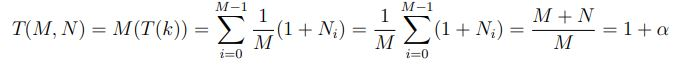
\includegraphics{images/76-83_mathwait}
$\blacksquare$

\setcounter{section}{77}
\section{Universal Hashing, математическое ожидание длины цепочки, содержащей фиксированный элемент.}
\textbf{Universal Hashing}. H - семейство хеш-функций универсально, если $\forall x \neq y \in U P_h(h(x) = h(y)) \leqslant 1/m$ - сильная универсальность, слабая универсальность - если это {O}(1/m); h - равномерно выбрана из (с вероятностью 1/мощность H). \par
Тогда суть в том, что выбирая случайную хеш-функцию из этого семейства, мы получаем не так много коллизий. Все оценки делаются по элементам, если мы выбираем случайную хеш-функцию, а не по фиксированной хеш-функции считаем что-либо. \par

\setcounter{section}{78}
\section{Пример универсального семейства хеш-функций (с доказательством): ((ax + b) mod p) mod m.}
\textbf{Universal Hashing}. H - семейство хеш-функций универсально, если $\forall x \neq y \in U P_h(h(x) = h(y)) \leqslant 1/m$ - сильная универсальность, слабая универсальность - если это {O}(1/m); h - равномерно выбрана из (с вероятностью 1/мощность H). \par
\textbf{Пример универсального семейства:} Допустим, что наши функции параметризуются. Тогда $H = \{ h_{\alpha, \beta}| h(x) = ((\alpha x + \beta)$ mod $p)$ mod $m\}$, где m - количество "бакетов" из таблицы, а p - некое большое простое число, >m. 
Таким образом, мы сокращаем хранение на затраты памяти от |U| log (m) до двух чисел (2 log(p)). \par
Докажем, что это семейство универсальное: $\forall x \neq y \in F_p$ ($F_p$ - поле по модулю p): $P_{\alpha, \beta}(h_{\alpha, \beta}(x) = h_{\alpha, \beta}(y))$, $\alpha \neq 0$. \par
1) $\alpha x + \beta = \alpha y + \beta$ - невозможно, т.к. иначе можно перенести правую часть влево и получить делители нуля, которых в поле нет. Все равенства - по модулю p. Отсюда следует, что после первого деления все числа различны. (Мы рассматриваем хеш-функцию как двухуровневую). Рассмотрим первый уровень детальнее: \par
2) Докажем, что любой элемент во второй таблице u на v (после деления mod m) можно получить: \par
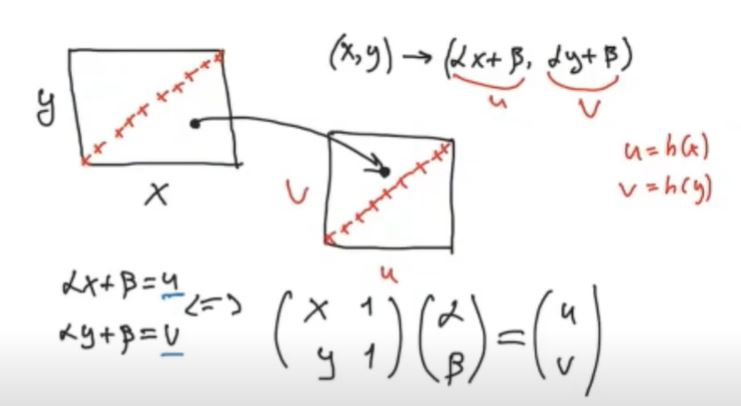
\includegraphics{images/76-83_biection} \par
Наша функция при фиксированных альфа и бета - инъекция, таким образом, любую пару (u; v) можно получить. Утверждение: $\forall x \neq y \exists \alpha, \beta:  h_{\alpha, \beta}(x) = u,  h_{\alpha, \beta}(y) = v$. Таким образом, у нас есть две фиксированные матрицы, а одну надо найти (которая из альфа и бета). Из линала: решение единственное, если определитель матрицы слева ненулевой: det = $x - y \neq 0$. \par
Из того, что любой паре (x, y) может сопоставляться любая пара $(\alpha, \beta)$, а все выборы делаются равномерно, можно сделать вывод, что $P_{\alpha, \beta}(h_{\alpha, \beta}(x) = h_{\alpha, \beta}(y)) = P_{u, v}(u$ mod $m = v$ mod $m)$. Теперь нам нужно оценить вероятность для $u \neq v$. \par
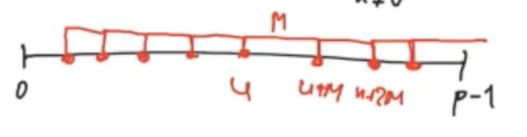
\includegraphics{images/76-83_segment_field} \par
Тут мы поставили u и прибавляем m в большую и меньшую стороны до p-1. При этом u не может подходить для v, т.к. $u \neq v$, а остальные точки, полученные таким образом - подходящие варианты v. Тогда: $P_{u, v}(u$ mod $m = v$ mod $m) \leqslant p \cdot (p/m -1)/(p(p-1))$, где p/m округляется вверх. -1 в числителе, т.к. пара (u, u) не может быть. $p \cdot (p/m -1)/(p(p-1)) \leqslant ((p+m-1)/m - 1)/(p-1)$ (это оценка для p/m, округлённого вверх). Осталось лишь внести -1 в числитель. Ч.т.д.

\setcounter{section}{79}
\section{Совершенное хеширование (задача Fixed Set), алгоритм FKS Hashing. Лемма о линейности математического ожидания времени построения совершенной хеш-таблицы.}
\textbf{Задача Fixed Set, совершенное хэширование} хочет добиться того, чтобы все операции работали за O(1) всегда, а не усреднённо. Вводим операцию Build($a_1, a_2, \dots, a_n$) - строит хеш-таблицу, а дальше есть только запросы find(x) - всё это работает за O(1) "честно", хотя Build работает за O(n) в среднем (и O(n) памяти). Идея: вместо цепочек использовать новые хеш-таблицы в каждом бакете, но тогда нам придётся подбирать нужные функции сначала для внешней хеш-таблицы ($h_{out}$, потом для внутренних ($h_i, h_j$) \par
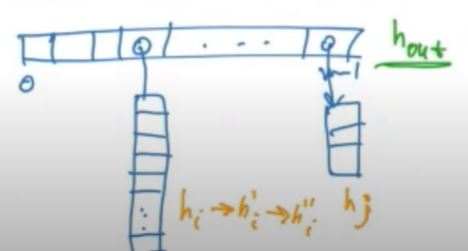
\includegraphics{images/76-83_perfect hash} \par
Мы требуем $h_i$ без коллизий. \par
\textbf{Лемма:} Если во внутреннюю таблицу попадает k элементов, то если взять хеш-таблицу размера $2k^2$, то вероятность существования хотя бы одной коллизии меньше 1/2. \par
$\blacktriangle$
$E \#$ коллизий $ = \sum_{x_l, x_m \in Bucket_i} P(h_i(x_l) = h_i(x_m)) \leqslant k(k-1)/(2k^2) \leqslant 1/2$ (первое неравенство вылезает из того, что вероятность совпадения хеш-функций равно 1/число бакетов).
$\blacksquare$ \par
$P(\# \text{коллизий} \geqslant 1) \leqslant E \#\text{коллизий} / 1 \leqslant 1/2$ (неравенство Маркова, б/д: $P(x \geqslant a) \leqslant E x / a$ при $a > 0$).

Тогда идея: если несколько раз попробовать найти функцию без коллизий, то скоро это получится. Теперь посмотрим на аналогичное для внешней хеш-таблицы. \par
Итак, при условии $m \geqslant n^2$, n элементов, P(у h нет коллизий) $\geqslant$ 1/2. Тогда размер каждой внутренней хеш-таблицы должен быть $\geqslant k^2$, где k - количество элементов в бакете. Тогда мы хотим, чтобы размеры всех внутренних таблиц были {O}(n): $\sum_{i=1}^M |C_i|^2 = {O}(n)$. Положим M=n. Мы хотим: $P(\sum_{i=1}^M |C_i|^2 \leqslant 4n) \geqslant 1/2$ (Последнее неравенство доказываем). 
$\blacktriangle$
h - выбираем равномерно из некоторого универсального семейства H. $E(\sum_i |C_i|^2) = $ \\
$= E(\sum_i |C_i|\cdot |C_i -1| /2 \cdot 2 + |C_i|) = N + 2E$ \# коллизий; N - число элементов. Осталось посчитать мат. ожидание числа коллизий: $\sum_{i < j} P(h(x_i) = h(x_j)) = N(N-1)/(2M)$, т.к. h выбирается из универсального семейства. Тогда $E(\sum_i |C_i|^2) = N + N(N-1)/M \leqslant 2N$ при M = N. Применим неравенство Маркова: $P(\sum_i |C_i|^2 > 4N) \leqslant E \sum_i |C_i|^2 /4N \leqslant 2N/4N = 1/2$. Но тогда $P(\sum_i |C_i|^2 \leqslant 4N) \geqslant 1/2$
$\blacksquare$ \par
\textbf{Лемма:} $\xi_1, \dots, \xi_n$ - независимые случайные величины, которые принимают значения либо 0, либо 1, и $\forall k p(\xi_k = 0) \leqslant p \in (0, 1)$. Пусть $\eta$ - первый номер, когда $\xi_{\eta} = 1$, тогда $E \eta \leqslant 1/(1-p)^2$ \par
0) P($\eta = \inf$) = $\prod{k=1}^{\inf} P(\xi_k = 0) \leqslant$ lim $_{k \rightarrow \inf P^k = 0}$ \par
1) E $\eta = \sum_{k=1}^{\inf} k P(\eta_1 = \dots = \eta_{k-1} = 0, \eta_k = 1) \leqslant \sum_{k=1}^{\inf} p^{k-1}k = (1/(1-x))'|_{x=p} = 1/(1-p)^2$; p = 1/2 $\Rightarrow $E $\eta \leqslant 4$ - мат. ожидание выбора внешней хеш-функции.
Мат. ожидание поиска внутренних хеш-функций: 4n, где n - количество бакетов, отсюда следует линейность алгоритма. \par
Минусы такой таблицы: мы не умеем её перестраивать. Это алгоритм Michael Fredman; János Komlós; Endre Szemerédi \textbf{FKS - алгоритм}. (было статическое хеширование, там динамическое).
\setcounter{section}{80}
\section{Открытое хеширование: линейное/квадратичное пробирование, двойное хеширование.}
\textbf{Хеш-таблицы с открытым ключом}: коллизии разрешаем, кладя элемент в следующий хеш. \\
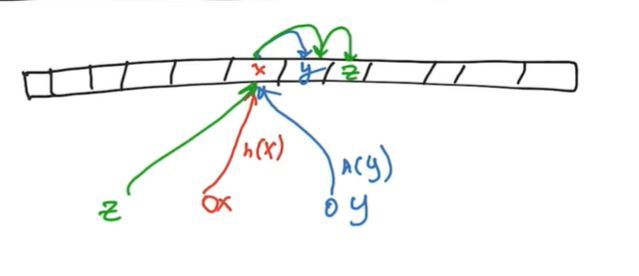
\includegraphics{images/76-83_open key} \par
Insert: идти направо, пока не найдёт первую дырку, туда вставляет \par
Find: аналогично insert: до первой дырки. \par
Чтобы удалить, нужно сначала локализовать, а потом удалить, но если его просто так удалить, то появляется "лишняя" дырка. Поэтому delete выполняется как locate (находим) + ставим tombstone ("могильный камень"): значение, которое не является "дыркой", означает, что там когда-то был элемент, но за ним могут быть идти другие элементы с тем же хешом. Тогда Insert считает tombstone за дырку, но если нужна проверка на повторы, то идти "до конца". \par
Таблица относительно скоро заполнится, надо будет делать rehash: как только количество будет выше порога, увеличиваем размер в два раза. \par
Сверху описана стратегия \textbf{линейного пробирования}: при поиске/вставке/удалении элемента идти вправо по одному, рассматривая ячейки и проверяя, что там лежит (другой элемент, дырка, tombstone): run$_i = (h(x) + i \% M)$. Существует \textbf{квадратичное пробирование}: run$_i = (h(x) + i^2 \% M)$. Здесь run - это зелёные стрелочки на рисунке, итерации при работе с элементами с одним хешем. Третий способ: \textbf{двойное хеширование} - мы заводим две хеш-функции, run$_i = (h_1(x) + i h_2(x)) \% M$

\setcounter{section}{81}
\section{Определение k-независимого семейства, зависимость асимптотик операций от типа семейства, из которого выбирается хеш-функция и вида пробирования (б/д).}
Универсальное семейство хеш-функций рассмотрено ранее; существует также понятие \textbf{k-независимое семейство}, которое является более сильным: $\forall x_1 \neq x_2 \neq \dots \neq x_k: $ случайные величины $h(x_1), h(x_2), \dots, h(x_k)$ - независимы в совокупности, т.е. при любой фиксации всех остальных хеш-функций $h(x_k)$ может принимать любые значения. \par
Таблица для k-независимых семейств в зависимости от k: \par
\begin{center}
\begin{tabular}{ |c|c|c|c| } 
 \hline
 - & 1. Лин. пробир. & 3. Двойное хеширование \\ 
 \hline
  k = 2 &  {O}($\sqrt{n}$) & O(1) \\ 
 \hline
  k = 3 &  {O}(log(n)) & - \\ 
 \hline
  k = 5 &  {O}(1) & - \\ 
 \hline
\end{tabular}
\end{center} \par
P.S. для двойного хеширования оба берутся из k=2.

\setcounter{section}{82}
\section{Фильтр Блума: идея. Оптимальные значения k при фиксированных n и m (б/д). Оптимальные k и m при фиксированных n и FPR (б/д).}
\textbf{Идея фильтра Блума:} хотим делать всё с той же асимптотикой, но с меньшей памятью. Надо чем-то пожертвовать: жертвуем корректностью. Пусть у нас есть множество, в котором мы хотим делать insert и find(x) (для find: где x лежит в множестве и x не лежит в множестве. Первый вариант - всегда точно отвечает, второй вариант - можно позволить ошибку вида "сказать да" с маленькой вероятностью (около 0,1\%). \par
\textbf{Пример}: spellchecker, работающий на базе данных. Строим промежуточный фильтр: присылаем запрос, если ответ "нет", то тогда гарантированно не надо идти в базу данных, если ответ "да", то можно обратиться в базу данных для дополнительной проверки. \par
\textbf{Устройство фильтра Блума:} прослоечка из k функций и большой массив бит от 0 до m-1. Запрос insert x: считаем каждую из хеш-функций от х, ставим туда, куда ведёт хеш, единицу. В случае коллизии при insert лишнюю единицу ставить не нужно. Find - нужно посчитать все k значений функции и проверить, что все k значений равны 1. Тогда если k лежит в множестве, там точно будут все единицы. иначе есть шанс ошибки. \par
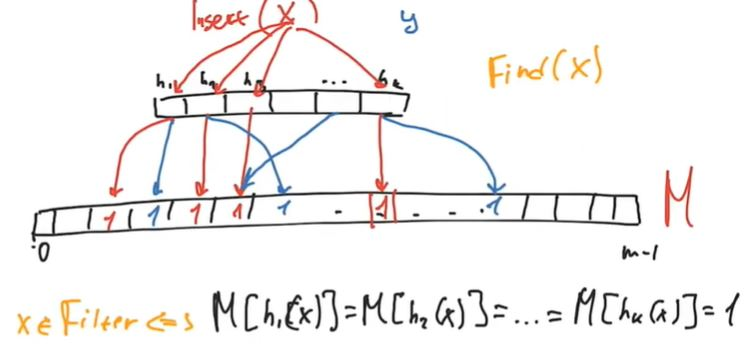
\includegraphics{images/76-83_bloom filter.JPG} \par
k функций, m бит, n ключей. P(j-й бит равен 1 после вставки всех ключей) $= 1 - P(=0) = 1 - P(h_1(x) \neq j) \cdot P(h_2(x) \neq j) \cdot \dots = 1 - (1 - 1/m)^{k \cdot n}$. Для конкретного элемента нужно возвести это всё в степень k: $(1 - (1 - 1/m)^{k \cdot n})^k$ - вероятность того, что k независимых бит равны единице. Это и есть та вероятность, с которой мы для y, не лежащего в таблице, выдаём ответ "да". (неверно, что значения этих k бит независимы, но мы закроем на это глаза, потребуем только, чтобы $h_{i_1}(x) \neq h_{i_2}(x), i_1 \neq i_2$). Если n и m фиксированные, то оптимальное k минимизирует величину FPR = $(1 - (1 - 1/m)^{k \cdot n})^k$ - False Positive Rate. Чтобы посчитать k, нужно взять производную, $k = m \cdot ln(2)/n$. Если даны n и $\varepsilon$ - желаемый FPR, то получаем оценки $m = -n ln(\varepsilon)/(ln 2)^2$, $k = - ln(\varepsilon)/ln 2$. Отсюда m/n = $\approx 1,44 log_2(\varepsilon)$ - количество бит на один элемент, близка к теоретическому минимуму. Фильтры сравнивают по этому значению. \par
Другие примеры фильтров: фильтр кукушки, XOR - фильтр (последний считается сейчас лучшим).